
\subsection{Memcached Performance}
\label{sec:eval:memcached}



%FIXME if different keys


\begin{figure*}[t]

\centering
  \vspace*{0.3in}
 \subfloat[Throughput for varying established connections]{
  \label{fig:connscaling:throughput}
   
\includegraphics[width=.49\textwidth,clip]{figs/blank.eps}}
 \hspace{.02in}
 \subfloat[Avg. and 99\% latency for varying established connections]{
  \label{fig:connscaling:lat}
  
\includegraphics[width=.49\textwidth,clip]{figs/blank.eps}}
\centering
  \vspace{-2.8in}
  \subfloat{
\includegraphics[width=1\textwidth,clip]{figs/short-key.eps}}
 \vspace{2.3in}
 \
\caption{Connection scaling}
 \label{fig:connscaling}

\end{figure*}

\begin{figure*}
\begin{centering}
\subfloat[Latency vs throughput for the memcached ETC workload.]{
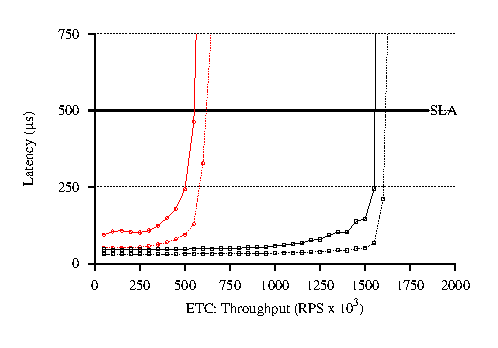
\includegraphics{figs/memcached-etc-basic.eps}}
\subfloat[Multilate-Me Again!]{

\includegraphics{figs/blank.eps}}
\caption{Capacity and quality of service of memcached on Linux and \ix for XXX and YYY concurrent, established connections}
\label{fig:mutilate}
\end{centering}
\end{figure*}



Finally, we evaluated the performance benefits of the \ix protected
dataplane design with \texttt{memcached}, a massively deployed,
in-memory key-value store built on top of the \texttt{libevent}
framework~\cite{url:memcached}. It is frequently used as a
high-throughput, low-latency caching tier in front of persistent
database servers. \texttt{memcached} is a network-bound
application, with threads spending over 80\% of execution time in
kernel mode for network processing~\cite{Leverich:RHSU:2014}. It is a
difficult application to scale, in particular because the
common deployments involve high connection counts for
\texttt{memcached} servers and small-sized requests and
replies~\cite{nishtala2013scaling,Atikoglu:2012:WAL}

We use the \texttt{mutilate} load-generator to place a selected load
on the server in terms of requests per second (RPS) and measure
response latency~\cite{url:mutilate}. \texttt{mutilate} coordinates a
large number of client threads across multiple machines to generate
the desired RPS load, while a separate unloaded client measures
latency by issuing one request at the time.  We configure
\texttt{mutilate} to generate load representative of two workloads
from Facebook~\cite{Atikoglu:2012:WAL}: the ETC workload that
represents that highest capacity deployment in Facebook, has 20B - 70B
keys, 1B-1KB values, and 90\% GET requests; and the USR workload that
represents deployment with most GET requests in Facebook, has short
keys ($<$20B), 2B values, and 99\% GET requests. In USR, almost all
traffic involves minimum-sized TCP packets. Each request is issued 
\dm{incomplete sentence?}

\dm{Paragraph needs editing.  Also, why not report 99\% or 99.9\%?}
\adam{Are our linux graphs too noisy to do 99th? IX looks fine at 99th...}
For all experiments, we report 95th percentile latency as a function
of the achieved throughput as this is the relevant metric for
datacenter
applications\microsecond~\cite{DBLP:journals/cacm/DeanB13}. This graph
provides insights the full range of system behaviors. Most commercial
\texttt{memcached} use such a latency-throughput graph to provision
each server so that the 95th percentile latency does not exceed 200 to
500.  We carefully tune the Linux baseline setup according to the
guidelines in \cite{Leverich:RHSU:2014}. Specifically, we pin
memcached threads, configure interrupt-distribution based on
thread-affinity, and tune interrupt moderation thresholds. We believe
that our baseline Linux numbers are as tuned as possible for this
hardware using the open-source version of
\texttt{memcached-1.4.18}. For our benchmark, we use 6 client machines
and a total of 772 connections to the memcached server. We report the
results for the configuration that provides the best performance: 
8 sockets with Linux, but only 6 with \ix.

\christos{Should we discuss the porting process to IX?}
\adam{new:} Porting memcached to IX primarly consisted of adapting it
to use our event library. In most cases, the port was straightforward,
replacing Linux and \texttt{libevent} function calls with their equivalent
versions in our API. There were a few incompatibilities that required
aditional effort. For example we don't yet support vectored write
operations (e.g., \texttt{writev}) in our
API (the benefits would be only marginal because we batch
writes inside our event library). Morever, we had to make some internal changes
to memcached in order to deliniate the spawning elastic threads and background
threads.  \adam{On our haswell machine, which runs an older linux
kernel this change works great, but it had to be disabled on the mavericks and at EPFL because
newer kernels have something wierd going on with thread spawning. In pratice,
background threads didn't make any noticable difference on the Haswell. Should I say anything about this
limitation?} Finally, we made some small changes to the behavior of the main
event loop in order to better support our run to completion execution model.


%%
%% see  figs/data/memcache-sla-qps.txt

%82.5  139.6  650K
%42.0  54.3   1320K  --> 2.03x     --> 2.0x
%79.6  136.8  580K
%37.7  44.5   1620K  -->  2.74519  --> 2.7x


\begin{table}[b]
%\vspace{-1em}
\begin{center}
\begin{small}
\begin{tabular}{|l|c|c|c|}
\hline
%Configuration &  \multicolumn{2}{|c|}{Unloaded latency} &  QPS for SLA:\\
Configuration &  Minimum latency &  RPS for SLA:\\
&  @99th pct &  $<500$\microsecond@99th pct\\
\hline
ETC-Linux & 93\microsecond & 500K\\
ETC-IX    & 46\microsecond & 1500K\\
\hline
USR-Linux & 84\microsecond & 450K\\
USR-IX    & 31\microsecond & 2150K\\

\hline
\end{tabular}
\caption{Unloaded latency and maximum RPS for a given service-level agreement for the memcache workloads \texttt{ETC} and \texttt{USR}.}
%\vspace*{-2em}
\label{tbl:mutilate}
\end{small}
\end{center}
\end{table}



\edb{NEW with table:} Fig.~\ref{fig:mutilate} shows the throughput-latency curves for the
two \texttt{memcached} workloads for Linux and \ix, while
Table~\ref{tbl:mutilate} reports the unloaded latencies and maximum query throughput that meets a service-level agreement of $<1ms$ at the 95th percentile.
\ix noticeably reduces the unloaded latencies, also measured
at the 95th percentile.  We note here that the benchmark
clients are running on Linux, and that running them on \ix should
further reduce that latency. 

\edb{NEW:}For both workloads, the distribution of CPU time shifts from being
$>80\%$ in the kernel with Linux to $<30\%$ with \ix.  Since the
application is unmodified, Amdahl's law would predict a speedup of 3x.
\ix actually increases the throughput of memcached by 1.8 and 2.7
for \texttt{ETC} and \texttt{USR}, respectively.  We explain the
difference by the increased lock contention within the application
itself, in particular for \texttt{ETC}, which has a higher write frequency.


%
\subsection{Multi-tier Performance}

\edb{THIS IS A STRECH STRETCH GOAL} 

Evaluating the performance of a highly-scalable, multi-tier
environment in a lab environment is challenging on multiple fronts:
first, there are ---to the best of our knowledge--- no universally
accepted multi-tier benchmarks that involve key-value stores and in
general that are representative of web-scale applications.  Second,
most lab enviornments are orders of magnitude smaller than a
datacenter.

Therefore, we construct a simple, synthetic multi-tier benchmark that
mimics the behavior of a social application stored in an in-memory
key-value store.  The application is a simple \texttt{http} server
that returns the top-most recent update among a users list of friends.
The application server parses the http request to
get the userid, uses the user id to return a friends-list from a
key-value store, and then queries the key-value store individually for
each friend for the most recent value.  It then processes replies and
return the top-most entries.  In our experiments, we model a database
with $10^7$ million users, each with 100 friends. 

We scale the benchmark to model a cluster deployment with $\alpha$
client connections per application server, $\beta$ httpd and $\gamma$
memcached servers.  Keys are distributed uniformly between the
$\gamma$ servers.  We model a large-scale deployment with
$\alpha=10^5$, $\beta=10^4$ and $\gamma=10^4$ on a deployment that consists of 4
actual application servers and 1 memcached server (running on our
server hardware with 4x10GbE connectivity).  Each application server
runs \texttt{lighthttpd} with the application logic written directly
within the server, and maintains a distinct connection for each of the
$\alpha$ virtual clients and $\gamma$ virtual nodes.  The key-value store is
running \texttt{memcache} as described in \S\ref{sec:eval:memcache}.
We use the remaining 14 client machines to simulate $4 \times \alpha$
clients and the 19th client to measure the latency of the application.

Fig.~\ref{missing} reports the latency as a function of the
throughput, as determined by varying the client load.  We compare a
Linux baseline with one in which \ix is used to run both the
application server and the memcached server.  We note that the choice
of operating system on the application server determines the number of
concurrent connections. Indeed, because of the coherence-free
execution model, each application server needs to open a distinct TCP
flow to the same virtual node for each of its hardware threads.

\edb{OPTIMISTIC: } Fig.~\ref{missing} shows that \ix can saturate the
hardware connectivity.  Indeed, the bottlneck consits of the
communication 






